%Jennifer Pan, August 2011

\documentclass[10pt,letter]{article}
	% basic article document class
	% use percent signs to make comments to yourself -- they will not show up.

\usepackage{amsmath}
\usepackage{amssymb}
	% packages that allow mathematical formatting

\usepackage{graphicx}
	% package that allows you to include graphics

\usepackage{enumitem}

\usepackage{setspace}
	% package that allows you to change spacing

\onehalfspacing
	% text become 1.5 spaced

\usepackage{fullpage}
	% package that specifies normal margins

\renewcommand{\vector}[1]{\boldsymbol{#1}}
\newcommand{\problem}[1]{\section*{Problem #1}}
\newcommand{\problempart}[1]{\paragraph{#1}}

\begin{document}
	% line of code telling latex that your document is beginning


\title{Problem Set 4}

\author{Nicholas Wu}

\date{Fall 2020}
	% Note: when you omit this command, the current dateis automatically included

\maketitle
	% tells latex to follow your header (e.g., title, author) commands.
\textbf{Note:} I use bold symbols to denote vectors and nonbolded symbols to denote scalars. I primarily use vector notation to shorthand some of the sums, since many of the sums are dot products.

\problem{1}

\problempart{(1)}
A rational expectations recursive equilibrium for this economy consists of pairs of functions for groups 1 and 2 describing the laws of motion $\mathcal{G}^A$ and $\mathcal{G}^B$, household value functions $V^A$ and $V^B$, household savings policy functions $g^A$ and $g^B$ (where we denote the first two arguments as the given sequences of capital and the last argument as the previous capital realization), interest rate function $R$, wage function $W$, such that the following conditions hold:
\begin{itemize}
\item Household optimization for $A$: $V^A$, $g^A$, solve the following household optimization:
\[ V^A(K^A, K^B, a; \mathcal{G}^A, \mathcal{G}^B) = \max_{a'} u(c) + \beta^A V^A(K'^A, K'^B, a'; \mathcal{G}^A, \mathcal{G}^B) \]
subject to
\[ c = R(K)a + W(K) - a' \]
\[ a, a' \ge \underline{A} \]
\[ K = \mu K^A + (1-\mu)K^B \]
\[ K'^A = \mathcal{G}^A(K^A, K^B) \]
\[ K'^B = \mathcal{G}^B(K^A, K^B) \]
where the optimal policy is
\[ a' = g^A(K^A, K^B, a; \mathcal{G}^A, \mathcal{G}^B )\]
\item Household optimization for $B$: $V^B$, $g^B$, solve the following household optimization:
\[ V^B(K^A, K^B, a; \mathcal{G}^A, \mathcal{G}^B) = \max_{a'} u(c) + \beta^B V^B(K'^A, K'^B, a'; \mathcal{G}^A, \mathcal{G}^B) \]
subject to
\[ c = R(K)a + W(K) - a' \]
\[ a, a' \ge \underline{A} \]
\[ K = \mu K^A + (1-\mu)K^B \]
\[ K'^A = \mathcal{G}^A(K^A, K^B) \]
\[ K'^B = \mathcal{G}^B(K^A, K^B) \]
where the optimal policy is
\[ a' = g^B(K^A, K^B, a; \mathcal{G}^A, \mathcal{G}^B )\]
\item Consistency with expectations:
\[ g^A(K^A, K^B, K^A; \mathcal{G}^A, \mathcal{G}^b) = \mathcal{G}^A(K^A, K^B)\]
\[ g^B(K^A, K^B, K^B; \mathcal{G}^A, \mathcal{G}^b) = \mathcal{G}^A(K^B, K^B)\]
\item Market clearing: (where $K = \mu K^1 + (1-\mu)K^2$)
\[ W(K) = (1-\alpha)\theta K^\alpha \]
\[ R(K) = \alpha \theta K^{\alpha-1} + 1- \delta \]
\end{itemize}
\problempart{(2)}
Due to the asset holding constraint $\underline{A}$, the Euler conditions are:
\[ u'(c^A) \ge \beta^A R(K) u'(c'^A) \]
\[ u'(c^B) \ge \beta^B R(K) u'(c'^B) \]
At steady state, $c^A = c'^A$ and $c^B = c'^B$, so we get
\[1 \ge \beta^A R(K) \]
\[ 1 \ge \beta^B R(K) \]
But we know $\beta^A > \beta^B$, and we cannot have both be strict inequality (else both consumers go to $\underline{A}$ for their asset holdings), so we must have
\[1 = \beta^A R(K) \]
\[1 > \beta^B R(K) \]
This implies that the steady state asset holding of consumers in group $B$ is: $A^B_{ss} = \underline{A}$. For group $A$, we have
\[ \frac{1}{\beta^A} = \alpha \theta K^{\alpha-1} + 1-\delta \]
So we can solve for the aggregate capital level:
\[ K_{ss} = \left(\frac{1}{\alpha\theta \beta^A} - \frac{1-\delta}{\alpha\theta}\right)^{1/(\alpha-1)}  \]
Then since
\[ \mu A^A_{ss} + (1-\mu)A^B_{ss} = K_{ss} \]
\[ A^A_{ss} = \frac{1}{\mu}\left(\frac{1}{\alpha\theta \beta^A} - \frac{1-\delta}{\alpha\theta}\right)^{1/(\alpha-1)} - \frac{1-\mu}{\mu}\underline{A} \]
\problempart{(3)} See attached file for code, and Figure 1 for the plot. Note that since $g_A$ essentially coincides with the  45 degree line, consumers in group $A$ essentially will consume the same consumption as the previous period at steady state, while the consumers in group $B$ will always consume less and less until they consume the minimum $\underline{A}$.

\begin{figure}
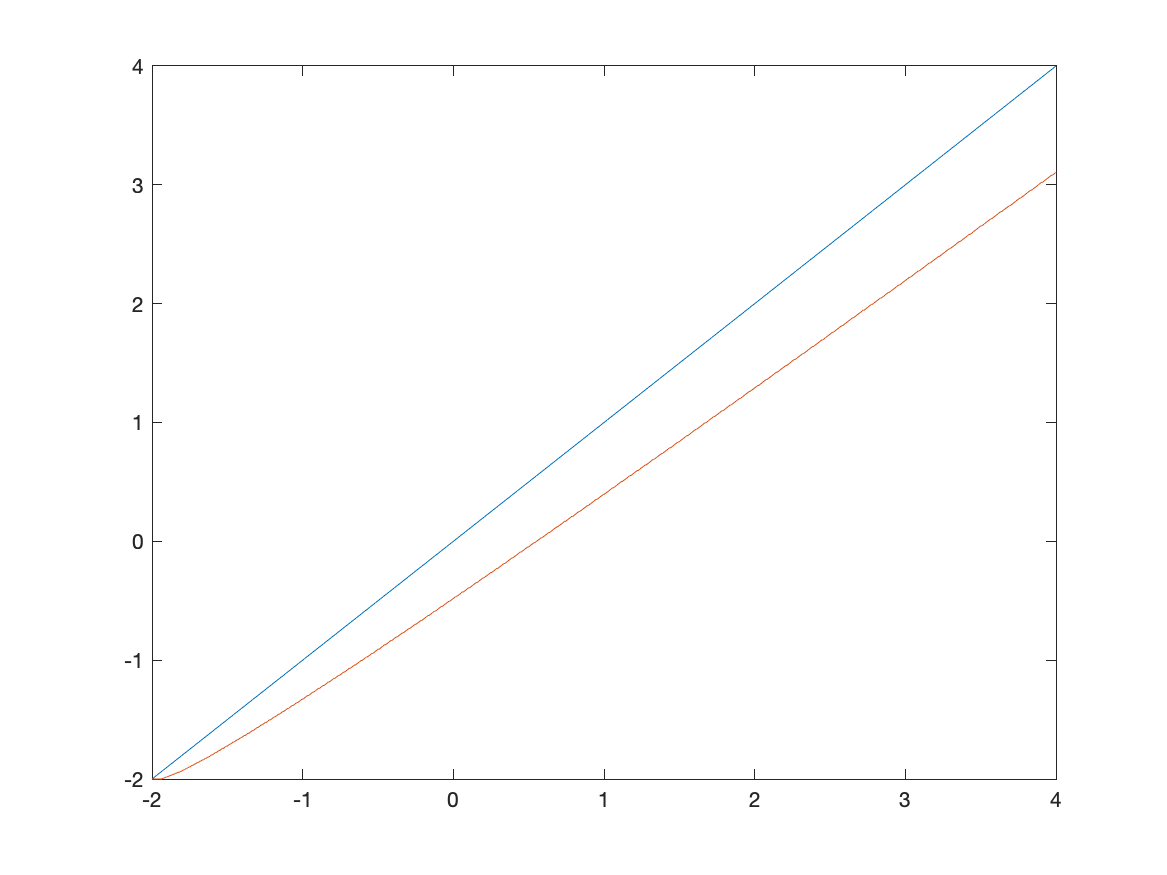
\includegraphics[scale=0.8]{ps4q1}
\caption{Heterogenous preferences: Blue line shows $g_A$, red line shows $g_B$. Note blue line essentially coincides with the 45 degree line.}
\end{figure}

\pagebreak
\problem{2}
\problempart{(1)}
A rational expectations recursive equilibrium for this economy consists of pairs of functions for groups A and B describing the laws of motion for capital $\mathcal{G}^A$ and $\mathcal{G}^B$, law of motion for supply $\mathcal{H}$, household value functions $V^A$ and $V^B$, household savings policy functions $g^A$ and $g^B$ (where we denote the first two arguments as the given sequences of capital and the last argument as the previous capital realization), labor policy functions $h^A$ and $h^B$ interest rate function $R$, wage function $W$, such that the following conditions hold:
\begin{itemize}
\item Consumers of type A optimize: $g^A, h^A, V^A$ solve:
\[ V^A(K^A, K^B, a; \mathcal{G}^A, \mathcal{G}^B, \mathcal{H}) = \max_{a', n} u(c, n) + \beta V^A((K^A)', (K^B)', a'; \mathcal{G}^A, \mathcal{G}^B, \mathcal{H}) \]
subject to:
\[ c = W(K, N)\epsilon_A n + R(K, N) a - a' \]
\[ K = \mu K^A + (1-\mu)K^B \]
\[ N = \mathcal{H}(K^A, K^B) \]
\[ (K^A)' = \mathcal{G}^A(K^A, K^B) \]
\[ (K^B)' = \mathcal{G}^B(K^A, K^B) \]
where $h^A$ defines the optimal policy for $n$ and $g^A$ describes the optimal policy for $a'$.
\item Consumers of type B optimize: $g^B, h^B, V^B$ solve:
\[ V^B(K^A, K^B, a; \mathcal{G}^A, \mathcal{G}^B, \mathcal{H}) = \max_{a', n} u(c, n) + \beta V^B((K^A)', (K^B)', a'; \mathcal{G}^A, \mathcal{G}^B, \mathcal{H}) \]
subject to:
\[ c = W(K, N)\epsilon_B n + R(K, N) a - a' \]
\[ K = \mu K^A + (1-\mu)K^B \]
\[ N = \mathcal{H}(K^A, K^B) \]
\[ (K^A)' = \mathcal{G}^A(K^A, K^B) \]
\[ (K^B)' = \mathcal{G}^B(K^A, K^B) \]
where $h^B$ defines the optimal policy for $n$ and $g^B$ describes the optimal policy for $a'$.
\item Consistency with expectations for capital and for labor:
\[ g^A(K^A,K^B, K^A; \mathcal{G}^A,\mathcal{G}^B, \mathcal{H}) = \mathcal{G}^A(K^A, K^B) \]
\[ g^B(K^A,K^B, K^B; \mathcal{G}^A,\mathcal{G}^B, \mathcal{H}) = \mathcal{G}^B(K^A, K^B) \]
\[ N = \mu \epsilon_A h^A(K^A, K^B, K^A; \mathcal{G}^A,\mathcal{G}^B, \mathcal{H}) + (1-\mu) \epsilon_B h^B(K^A, K^B, K^B; \mathcal{G}^A,\mathcal{G}^B, \mathcal{H}) = \mathcal{H}(K^A, K^B) \]
\item Market clearing prices:
\[ W(K, N) = (1-\alpha)\theta K^\alpha N^{-\alpha} \]
\[ R(K, N) = \alpha \theta K^{\alpha-1}N^{1-\alpha} + (1-\delta) \]
where
\[ K = \mu K^A + (1-\mu)K^B \]
\end{itemize}
\problempart{(2)}
From steady state in the Euler condition, after using the envelope theorem, $1 = \beta R(K,N)$ so we have:
\[ 1 = \beta \left( \alpha \theta K_{ss}^{\alpha-1}N_{ss}^{1-\alpha} + (1-\delta)\right) \]
We take the FOC of the maximizations with respect to $n$
\[ (1-\alpha)\theta K_{ss}^\alpha N_{ss}^{-\alpha}\epsilon_Au_1(c^A_{ss}, n^A_{ss})  + u_2(c^A_{ss}, n^A_{ss}) = 0 \]
\[ (1-\alpha)\theta K_{ss}^\alpha N_{ss}^{-\alpha}\epsilon_Bu_1(c^B_{ss}, n^B_{ss})  + u_2(c^B_{ss}, n^B_{ss}) = 0 \]
From expectation consistency:
\[ K_{ss} = \mu k^A_{ss} + (1-\mu) k^B_{ss} \]
\[ N_{ss} = \mu \epsilon_A n^A_{ss} + (1-\mu) \epsilon_B n^B_{ss} \]
Lastly, from the budget constraints, we get
\[ c^A_{ss} =  (1-\alpha)\theta K_{ss}^\alpha N_{ss}^{-\alpha} \epsilon_A n^A_{ss} + \left( \alpha \theta K_{ss}^{\alpha-1}N_{ss}^{1-\alpha} -\delta)\right) k^A_{ss} \]
\[ c^B_{ss} =  (1-\alpha)\theta K_{ss}^\alpha N_{ss}^{-\alpha} \epsilon_B n^B_{ss} + \left( \alpha \theta K_{ss}^{\alpha-1}N_{ss}^{1-\alpha} -\delta)\right) k^B_{ss} \]
The unknowns are $c^A_{ss}, c^A_{ss}, k^A_{ss}, k^A_{ss}, n^A_{ss}, n^A_{ss}, K_{ss}$, and $N_{ss}$, but we only have 7 equations. Hence this system has a spectrum of steady states. The aggregate capital level thus can vary, and there is no unique steady state level of aggregate capital.
\problempart{(3)}

A rational expectations recursive equilibrium for this economy consists of pairs of functions for groups A and B describing the laws of motion for capital $\mathcal{G}^A$ and $\mathcal{G}^B$, law of motion for aggregate labor supply $\mathcal{H}$, law of motion for labor supply of group $A$ $\mathcal{H}^A$, household value functions $V^A$ and $V^B$, household savings policy functions $g^A$ and $g^B$ (where we denote the first two arguments as the given sequences of capital and the last argument as the previous capital realization), labor policy functions $h^A$ and $h^B$ interest rate function $R$, wage function $W$, such that the following conditions hold:
\begin{itemize}
\item Consumers of type A optimize: $g^A, h^A, V^A$ solve:
\[ V^A(K^A, K^B, N^A, a, n; \mathcal{G}^A, \mathcal{G}^B, \mathcal{H},\mathcal{H}^A) = \max_{a', n'} u(c, n', n) + \beta V^A((K^A)', (K^B)', (N^A)', a', n'; \mathcal{G}^A, \mathcal{G}^B, \mathcal{H},\mathcal{H}^A) \]
subject to:
\[ c = W(K, N)\epsilon_A n' + R(K, N) a - a' \]
\[ K = \mu K^A + (1-\mu)K^B \]
\[ N = \mathcal{H}(K^A, K^B, N^A) \]
\[ (K^A)' = \mathcal{G}^A(K^A, K^B, N^A) \]
\[ (K^B)' = \mathcal{G}^B(K^A, K^B, N^A) \]
\[ (N^A)' = \mathcal{H}^A(K^A, K^B, N^A) \]
where $h^A$ defines the optimal policy for $n$ and $g^A$ describes the optimal policy for $a'$.
\item Consumers of type B optimize: $g^B, h^B, V^B$ solve:
\[ V^B(K^A, K^B, N^A, a; \mathcal{G}^A, \mathcal{G}^B, \mathcal{H},\mathcal{H}^A) = \max_{a', n} u(c, n) + \beta V^B((K^A)', (K^B)', (N^A)', a'; \mathcal{G}^A, \mathcal{G}^B, \mathcal{H},\mathcal{H}^A) \]
subject to:
\[ c = W(K, N)\epsilon_B n + R(K, N) a - a' \]
\[ K = \mu K^A + (1-\mu)K^B \]
\[ N = \mathcal{H}(K^A, K^B, N^A) \]
\[ (K^A)' = \mathcal{G}^A(K^A, K^B, N^A) \]
\[ (K^B)' = \mathcal{G}^B(K^A, K^B, N^A) \]
\[ (N^A)' = \mathcal{H}^A(K^A, K^B, N^A) \]
where $h^B$ defines the optimal policy for $n$ and $g^B$ describes the optimal policy for $a'$.
\item Consistency with expectations for capital and for labor:
\[ g^A(K^A,K^B, N^A, K^A; \mathcal{G}^A,\mathcal{G}^B, \mathcal{H},\mathcal{H}^A) = \mathcal{G}^A(K^A, K^B, N^A) \]
\[ g^B(K^A,K^B, N^A, K^B; \mathcal{G}^A,\mathcal{G}^B, \mathcal{H},\mathcal{H}^A) = \mathcal{G}^B(K^A, K^B, N^A) \]
\[ h^A(K^A, K^B, N^A, K^A; \mathcal{G}^A,\mathcal{G}^B, \mathcal{H},\mathcal{H}^A) = \mathcal{H}^A(K^A, K^B, N^A) \]
\[ N = \mu \epsilon_A h^A(K^A, K^B, N^A, K^A; \mathcal{G}^A,\mathcal{G}^B, \mathcal{H},\mathcal{H}^A) + (1-\mu) \epsilon_B h^B(K^A, K^B, N^A, K^B; \mathcal{G}^A,\mathcal{G}^B, \mathcal{H},\mathcal{H}^A) = \mathcal{H}(K^A, K^B) \]
\item Market clearing prices:
\[ W(K, N) = (1-\alpha)\theta K^\alpha N^{-\alpha} \]
\[ R(K, N) = \alpha \theta K^{\alpha-1}N^{1-\alpha} + (1-\delta) \]
where
\[ K = \mu K^A + (1-\mu)K^B \]
\end{itemize}
To argue efficiency, we consider the social planner problem:
\[ \Upsilon(K, N_A) = \max_{K', N_A', N_B'} \gamma u(C_A, N_A', N_A) + (1-\gamma) u(C_B, N_B') + \beta \Upsilon(K', N_A') \]
subject to:
\[ \mu C_A + (1-\mu)C_B + K' = \theta K^\alpha (\mu \epsilon_A N_A' + (1-\mu)\epsilon_B N_B')^{1-\alpha} + (1-\delta)K \]
We take $\gamma = \mu$, and then write the FOCs of this problem (applying the envelope theorem when necessary), where $\lambda$ is the Lagrange multiplier on the constraint:
\[ \mu u_1(C_A, N_A', N_A) - \mu \lambda = 0 \]
\[ (1-\mu) u_1(C_B, N_B) - (1-\mu) \lambda = 0 \]
\[ \beta \Upsilon_1(K', N_A') - \lambda = \beta \lambda (\alpha \theta K^{\alpha - 1}(\mu \epsilon_A N_A' + (1-\mu)\epsilon_B N_B')^{1-\alpha} + 1 - \delta )  - \lambda = 0 \]
\[ \mu u_2(C_A, N_A', N_A) + \beta \Upsilon_2(K', N_A') + \lambda (1-\alpha)\theta K^\alpha (\mu \epsilon_A N_A' + (1-\mu)\epsilon_B N_B')^{-\alpha}\mu\epsilon_A = \] \[ \mu u_2(C_A, N_A', N_A) + \beta \mu u_3(C_A, N_A', N_A) + \lambda (1-\alpha)\theta K^\alpha (\mu \epsilon_A N_A' + (1-\mu)\epsilon_B N_B')^{-\alpha}\mu\epsilon_A = 0 \]
\[ (1-\mu) u_2(C_B, N_B) + \lambda (1-\alpha)\theta K^\alpha (\mu \epsilon_A N_A' + (1-\mu)\epsilon_B N_B')^{-\alpha}(1-\mu)\epsilon_B = 0  \]
If we sub in the terms $R(K,N)$ and $W(K,N)$ determined by the market clearing conditions, we get
\[ u_1(C_A, N_A', N_A) =  \beta R(K', N') u_1(C_A', N_A'', N_A') \]
\[ u_1(C_B, N_B) =  \beta R(K', N') u_1(C_B', N_B') \]
\[ u_2(C_A, N_A', N_A) + \beta u_3(C_A, N_A', N_A) + W(K, N)\epsilon_A u_1(C_A, N_A', N_A) = 0 \]
\[ u_2(C_B, N_B) + W(K,N)\epsilon_B u_1(C_B, N_B) = 0 \]
But note that the first and third of these are exactly the FOC conditions for the maximization problem for consumer group $A$, and the second and fourth are exactly the FOCs for consumer group $B$. Hence, an equilibrium allocation also solves the social planner problem for $\gamma = \mu$, and hence is efficient. 

\pagebreak
\problem{3}
\problempart{(1)}
A rational expectations recursive equilibrium for this economy consists of pairs of functions for groups A and B describing the laws of motion for capital $\mathcal{G}^A$ and $\mathcal{G}^B$, household value function $V$, household savings policy function $g$, interest rate function $R$, wage function $W$, such that the following conditions hold:
\begin{itemize}
\item Consumers maximize: that is, $V, g$ solve the maximization problem
\[ V(K^A, K^B, a; \mathcal{G}^A, \mathcal{G}^b) = \max_{a'} \log(c) + \beta V((K^A)', (K^B)', a'; \mathcal{G}^A, \mathcal{G}^B) \]
where
\[ c = R(K)a + W(K) - a' \]
\[ a, a' \ge \underline{A} \]
\[ K = \mu K^A + (1-\mu) K^B \]
\[ (K^A)' = \mathcal{G}^A(K^A, K^B) \]
\[ (K^B)' = \mathcal{G}^B(K^A, K^B) \]
\item Consistency with expectations:
\[ g(K^A, K^B, K^A) = \mathcal{G}^A(K^A, K^B) \]
\[ g(K^A, K^B, K^B) = \mathcal{G}^B(K^A, K^B) \]
\item Market clearing:
\[ R(K) = \alpha \theta K^{\alpha - 1} + (1-\delta)\]
\[ W(K) = (1-\alpha)\theta K^{\alpha} \]

To characterize the steady state, we have from the Euler condition:
\[ \beta (\alpha \theta K_{ss}^{\alpha - 1} + (1-\delta)) = 1 \]
\[ \alpha \theta K_{ss}^{\alpha - 1} = \frac{1}{\beta} - (1-\delta) \]
\[ K^* = \left(\frac{\beta \alpha \theta}{1 - \beta(1 - \delta)} \right)^{1/(1-\alpha)}\]
\end{itemize}
\problempart{(2)}
To do this, we start by solving for $V, g$ using value function iteration, interpolating in the maximization term $\beta V((K^A)', (K^B)', a')$. We note that since the consumers all have homogeneous preferences, we only have to solve for a single policy function $g$. We further note that the dependence on $K^A$ and $K^B$ is only through $K$. That is, let us examine the maximization problem:
\[ V(K^A, K^B, a; \mathcal{G}^A, \mathcal{G}^b) = \max_{a'} \log(c) + \beta V((K^A)', (K^B)', a'; \mathcal{G}^A, \mathcal{G}^B) \]
where
\[ c = R(K)a + W(K) - a' \]
\[ a, a' \ge \underline{A} \]
\[ K = \mu K^A + (1-\mu) K^B \]
\[ (K^A)' = \mathcal{G}^A(K^A, K^B) \]
\[ (K^B)' = \mathcal{G}^B(K^A, K^B) \]

To solve for $g(k, K)$, we can use policy function iteration repeatedly and the result of exercise 4.4 from SLP that we did last week. Specifically, we can start from an arbitrary $\mathcal{G}^A_0, \mathcal{G}^B_0$, and use VFI to approximate the fixed point $V_0$ such that
\[ V_0(K^A, K^B, k) = \max_{k'} u(R(K)a + W(K) - k') + \beta V_0(k', \mathcal{G}^A_0(K^A, K^B), \mathcal{G}^B_0(K^A, K^B)) \]
Define $g_1$ then as the optimal policy of $V_0$, and subsequently $g_i$ as the optimal policy for $V_{i-1}$ and $V_i$ as the fixed point under the $\mathcal{G}^A, \mathcal{G}^B$ induced by $g_i$, then we exactly have the proposition of SLP exercise 4.4 part c. Hence we know $V_i$ will converge to the true fixed point. We can then use the following algorithm to find $V, g$:
\begin{enumerate}
\item Guess $\mathcal{G}^A, \mathcal{G}^B$.
\item Use PFI to find the optimal policy $g$ for $k'$ such that
\[ V(K^A, K^B, k) = \max_{k'} u(R(K)a + W(K) - k') + \beta V(\mathcal{G}^A(K^A, K^B),\mathcal{G}^B(K^A, K^B),k') \]
\item Update $\mathcal{G}^A(K^A, K^B) = g(K^A, K^B, K^A)$ and $\mathcal{G}^B(K^A, K^B) = g(K^A, K^B, K^B)$.
\item Go back to 2 and repeat until desired precision.
\end{enumerate}

We show our results for $\alpha = 0.4$, $\theta = 0.8$, $\mu = 0.5$, $\delta=0.3$, $\beta = 0.9$.

\begin{figure}
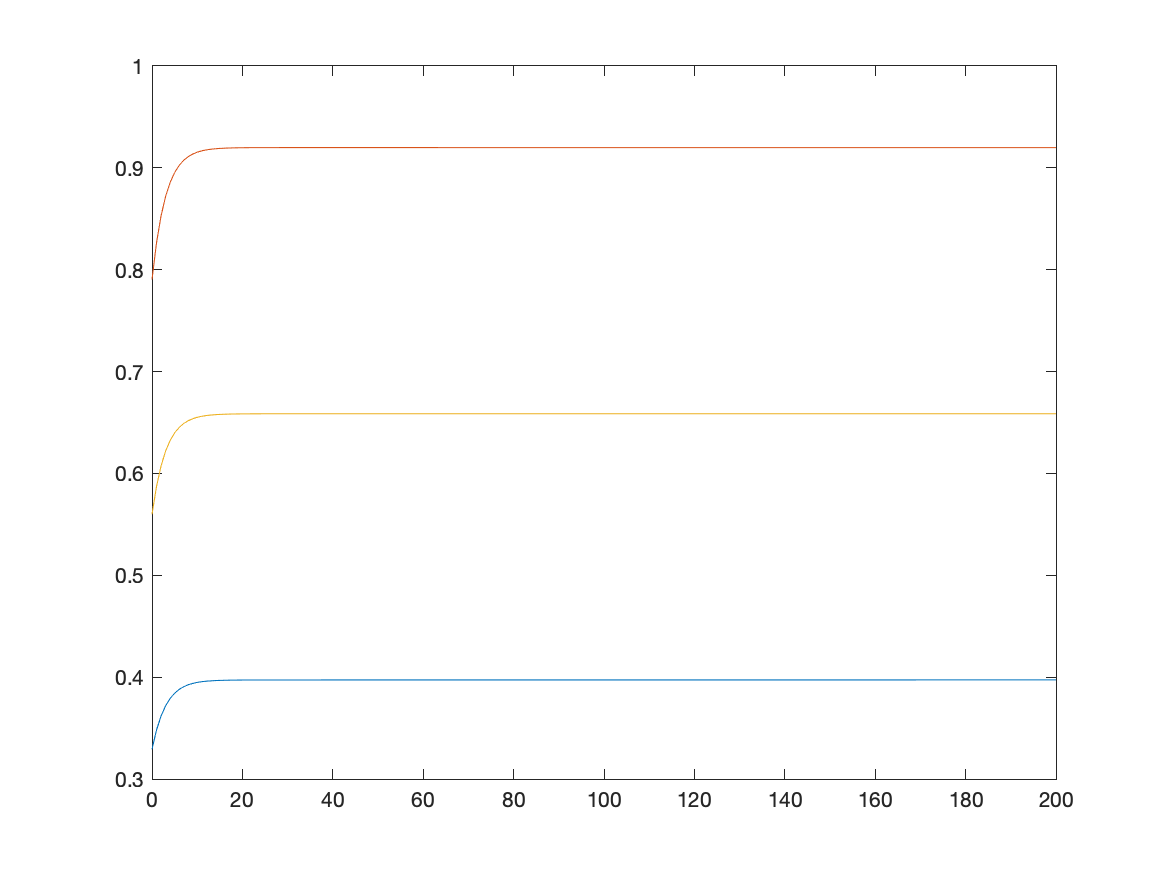
\includegraphics[scale=0.8]{ps4q3}
\caption{Heterogenous wealth. The richer type's capital sequence is in red, the poorer type in blue, and the aggregate capital in yellow. For these parameters, we note the aggregate capital sequence converges to its steady state.}
\end{figure}

\end{document}
	% line of code telling latex that your document is ending. If you leave this out, you'll get an error
